\section{Các thư viện cho ReactJs}

\subsection{Flux}
\begin{center}
  \captionsetup{type=figure}
  \includesvg[width=6cm]{img/flux-logo}
  \captionof{figure}{Flux}
\end{center}
\textbf{Giới thiệu:}

Flux là một kiến trúc phát triển ứng dụng mà Facebook sử dụng để hỗ trợ React. Flux giúp làm việc với các components của React một cách dễ dàng bằng cách sử dụng luồng dữ liệu một chiều (Unidirectional Data Flow). Giải pháp này khiến luồng dữ liệu trong ứng dụng luôn di chuyển theo 1 hướng duy nhất. Khi dữ liệu thay đổi, luồng này lại khởi chạy lại từ đầu.
\begin{center}
  \captionsetup{type=figure}
  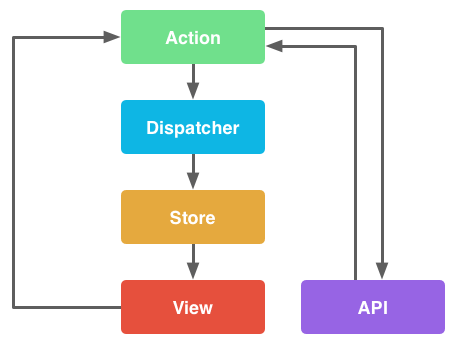
\includegraphics[width=14cm]{img/flux-flow}
  \captionof{figure}{Flux flow}
\end{center}

\textbf{Mô hình hoạt động của Flux:}
\begin{itemize}
    \item \textbf{View}: có nhiệm vụ hiển thị nội dung của ứng dụng (có thể hiểu giống như thành phần V trong mô hình MVC).
    
    Khi người dùng tương tác với ứng dụng làm thay đổi trạng thái (state) của ứng dụng (VD: thêm, sửa, xóa dữ liệu cá nhân), View sẽ thông qua Action gửi các thông tin thay đổi tới Dispatcher gồm có :
    \begin{itemize}
        \item action\_name: tên của Action (VD: ADD\_ITEM - thêm sản phẩm vào giỏ hàng).
        \item action\_payload: thông tin chi tiết nội dung muốn gửi (VD: Object chứa thông tin ID, quantity, price, ... của sản phẩm).
    \end{itemize}
    \item \textbf{Action}: Phát tán (dispatch) actions bằng Dispatcher đến những nơi đã đăng kí (register) nhận action đó.
    \item \textbf{Dispatcher}: Đối tượng trung gian, sau khi nhận được thông tin từ Action, Dispatcher làm nhiệm vụ truyền tải (broadcast) nội dung nhận được tới các Store đăng ký lắng nghe sự kiện thay đổi từ trước đó.
    \item \textbf{Store}: Trung tâm dữ liệu, sau khi nhận thông tin, Store tiến hành cập nhật dữ liệu (có thể hiểu việc cập nhật dữ liệu ở đây giống việc cập nhật state của Component). Sau khi cập nhật, Store bắn sự kiện xuống View để tiến hành cập nhật hiển thị cho người dùng.
    \item Ngoài ra trong sơ đồ trên còn có một thành phần API để lấy dữ liệu từ Remote Server.
\end {itemize}
Sơ đồ trên đảm bảo luồng dữ liệu di chuyển trong Flux bắt buộc đi theo một đường nhất định.

\subsection{Redux}
\begin{center}
  \captionsetup{type=figure}
  
\includegraphics[width=10cm]{img/redux-logo.png}
  \captionof{figure}{Redux}
\end{center}
\textbf{Giới thiệu:}
Do yêu cầu cho các ứng dụng single-page sử dụng Javascript ngày càng trở lên phức tạp thì code của chúng ta phải quản lý nhiều state hơn. Redux ra đời là một công cụ hỗ trợ cho các ứng dụng JavaScipt, giúp quản lý các trạng thái một cách khoa học và hiệu quả hơn.

Redux học hỏi kiến trúc của Flux nhưng nó lược bỏ đi sự phức tạp không cần thiết.
\begin{itemize}
    \item Redux không có khái niệm DISPATCHER.
    \item Redux chỉ có một STORE duy nhất thay vi nhiều STORE như của Flux.
    \item Các đối tượng Action sẽ được tiếp nhận và xử lý trực tiếp bởi STORE.
\end {itemize}
\textbf{Mô hình hoạt động của Flux:}
\begin{center}
  \captionsetup{type=figure}
  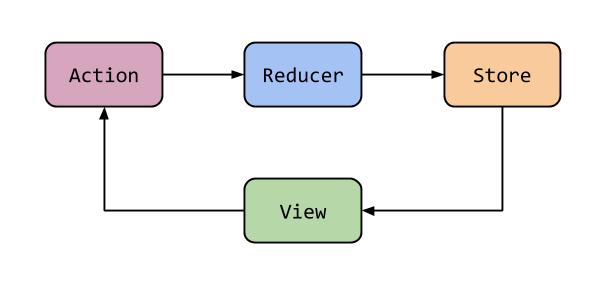
\includegraphics[width=10cm]{img/redux-architecture.png}
  \captionof{figure}{Redux architecture}
\end{center}
\begin{itemize}
    \item \textbf{Store}: Chứa state cho toàn bộ ứng dụng của bạn.
    \item \textbf{Reducers}: Lắng nghe các hành động (Actions) và thực hiện các thay đổi trên các giá trị của Store. Nó không thể biến đổi dữ liệu trên Store, nhưng phải trả lại một bộ dữ liệu mới (new data).
    \item \textbf{Actions}: Nó được định nghĩa như các khối thông tin (payloads) gửi dữ liệu từ ứng dụng của bạn đến Store. Chúng là nguồn thông tin duy nhất cho Store. Bạn có thể gửi chúng đến Store bằng cách sử dụng store.dispatch().
\end {itemize}
\subsection{Kết luận và lựa chọn}
Flux và Redux là hai công cụ hỗ trợ React được sử dụng phổ biến hiện nay. Tuy nhiên việc Redux ra đời sau và lấy cảm hứng từ kiến trúc Flux. Vì vậy, Redux mang nhiều ưu điểm được cải tiến từ Flux. Vậy nên khi sử dụng Redux sẽ đơn giản và ít gặp một số vấn đề khó giải quyết như khi sử dụng Flux.
Vì vậy nhóm quyết định sử dụng React kết hợp với Redux trong ứng dụng Phòng tổ chức hành chính.